\chapter{Một số dạng kiểm định thống kê}

\section{Kiểm định Pearson}

\subsection{Cơ sở lý thuyết}
\begin{dn}[Bài toán phù hợp phân phối (GOF)]
Cho một mẫu quan sát rời rạc được nhóm thành $r$ khoảng (bin) với số quan sát $O_i$ và xác suất kỳ vọng theo mô hình $p_i$ $(i=1,\ldots,r)$. Đặt $E_i=Np_i$ là tần số kỳ vọng. Thống kê kiểm định Pearson là
\[
\chi^2=\sum_{i=1}^{r}\frac{(O_i-E_i)^2}{E_i}.
\]
Khi $N$ đủ lớn và mọi $p_i>0$, dưới $H_0$ ta có $\chi^2\,\overset{d}{\approx}\,\chi^2(r-1)$.
\end{dn}

\begin{dn}[Kiểm định độc lập (bảng chéo $r\times c$)]
Với bảng số liệu $O_{ij}$ $(i=1,\ldots,r,\; j=1,\ldots,c)$, đặt tổng hàng $O_{i\cdot}$, tổng cột $O_{\cdot j}$ và $N=\sum_{i,j}O_{ij}$. Dưới giả thuyết “hàng và cột độc lập”, tần số kỳ vọng là $E_{ij}=\dfrac{O_{i\cdot}O_{\cdot j}}{N}$, và
\[\chi^2=\sum_{i=1}^{r}\sum_{j=1}^{c}\frac{(O_{ij}-E_{ij})^2}{E_{ij}}\,\overset{d}{\approx}\,\chi^2\big((r-1)(c-1)\big).
\]
\end{dn}

\begin{tinhchat}
- Điều kiện kinh điển để áp dụng: các quan sát độc lập; $E_i\ge5$ (GOF) hoặc $E_{ij}\ge5$ (bảng chéo) với phần lớn ô; kích thước mẫu đủ lớn.
- Quy tắc bác bỏ ở mức ý nghĩa $\alpha$: bác bỏ $H_0$ nếu $\chi^2>\chi^2_{1-\alpha,\,\nu}$ với bậc tự do $\nu$ tương ứng.
\end{tinhchat}

\subsection{Ví dụ GOF khác hoàn toàn}
Khảo sát $N=200$ người về màu yêu thích trong 4 màu: Đỏ, Xanh dương, Xanh lá, Vàng. Giả thuyết $H_0$: phân phối đồng đều ($p_i=0.25$). Dữ liệu quan sát: $O=(62,41,53,44)$. Khi đó $E_i=50$.

Tính
\[
\chi^2=\sum_{i=1}^{4}\frac{(O_i-50)^2}{50}=\frac{12^2}{50}+\frac{(-9)^2}{50}+\frac{3^2}{50}+\frac{(-6)^2}{50}=5.40.
\]
Với $\nu=3$ và $\alpha=0.05$, $\chi^2_{0.95,3}=7.815$. Vì $5.40<7.815$, \textbf{không bác bỏ} $H_0$. Ước lượng p-value $\approx0.145$.

\subsection{Ví dụ kiểm định độc lập khác hoàn toàn}
Nghiên cứu mối liên hệ giữa thói quen tập thể dục (Hàng ngày/Thỉnh thoảng) và tình trạng hút thuốc (Không hút/Đã bỏ/Hút hiện tại) trên $N=160$ người:
\[
O=\begin{array}{c|ccc}
 & \text{Không hút} & \text{Đã bỏ} & \text{Hút hiện tại}\\\hline
\text{Hàng ngày} & 48 & 22 & 10\\
\text{Thỉnh thoảng} & 36 & 28 & 16
\end{array}
\]
Từ đó $E=\begin{smallmatrix}(42,25,13)\\(42,25,13)\end{smallmatrix}$. Tính $\chi^2=3.82$ với $\nu=(2-1)(3-1)=2$. Vì $\chi^2_{0.95,2}=5.991$ nên \textbf{không bác bỏ} $H_0$ (p-value $\approx0.148$).

\subsection{Thực nghiệm số (MATLAB minh họa)}
\begin{matlab}
\begin{lstlisting}
function [chi2_stat, chi2_crit, pval] = pearson_gof_demo(N, bins)
% Minh họa GOF với phân phối rời rạc tùy chọn
Z  = 1:5;                         % các giá trị
PZ = [0.10 0.18 0.32 0.25 0.15];  % mô hình giả thuyết

% Sinh mẫu theo mô hình để so sánh (có thể thay bằng dữ liệu thực)
sample = randsrc(1, N, [Z; PZ]);
[O, edges] = histcounts(sample, bins, 'BinMethod','integers');
E = N * PZ(1:bins);               % đơn giản: ghép 5 bins = 5 xác suất

chi2_stat = sum((O - E).^2 ./ max(E, eps));
chi2_crit = chi2inv(0.95, bins - 1);
pval      = 1 - chi2cdf(chi2_stat, bins - 1);
end
\end{lstlisting}
\end{matlab}

\begin{figure}[h!]
    \centering
    
\includegraphics[width=.75\linewidth]{../../assets/logos/university-logo.png}
    \caption{Minh họa biểu đồ tần suất và CDF khi kiểm định Pearson}
\end{figure}

\section{Bộ hàm MATLAB kèm theo để chạy}
Các hàm dưới đây không phụ thuộc toolbox đặc biệt (tự cài ECDF và p-value Kolmogorov), có thể copy chạy trực tiếp.

\subsection{Sinh mẫu rời rạc và kiểm định Pearson (GOF)}
\begin{matlab}
\begin{lstlisting}
function [chi2_stat, df, p_value, O, E] = pearson_gof(z_vals, p_vec, N)
% Kiểm định Pearson phù hợp phân phối (GOF) cho biến rời rạc
% INPUT  z_vals: vector các giá trị có thể xảy ra (1 x m)
%        p_vec : vector xác suất tương ứng (1 x m), tổng = 1
%        N     : kích thước mẫu cần sinh (hoặc dữ liệu thực tế nếu có)
% OUTPUT chi2_stat: thống kê Chi-square
%        df       : bậc tự do m-1
%        p_value  : p-value
%        O, E     : tần số quan sát và kỳ vọng

% sinh mẫu theo (z, p)
s = discrete_rnd(z_vals, p_vec, N);

% đếm tần số theo từng hạng mục
m = numel(z_vals); O = zeros(1, m);
for i = 1:m
    O(i) = sum(s == z_vals(i));
end
E = N * p_vec(:)';

% thống kê chi-square và bậc tự do
chi2_stat = sum((O - E).^2 ./ max(E, eps));
df = m - 1;
p_value = 1 - chi2cdf(chi2_stat, df);
end

function s = discrete_rnd(z, p, N)
% Lấy mẫu rời rạc theo phân phối p trên tập giá trị z (không cần toolbox)
cp = cumsum(p(:));
u  = rand(N, 1);
idx = arrayfun(@(t) find(cp >= t, 1, 'first'), u);
s = z(idx);
end
\end{lstlisting}
\end{matlab}

\subsection{Kiểm định Pearson độc lập cho bảng chéo}
\begin{matlab}
\begin{lstlisting}
function [chi2_stat, df, p_value, E] = pearson_independence(O, alpha)
% Kiểm định độc lập hàng-cột cho bảng chéo O (r x c)
% O: ma trận tần số quan sát
% alpha: mức ý nghĩa (không bắt buộc)

if nargin < 2, alpha = 0.05; end
[r, c] = size(O);
N = sum(O(:));
E = (sum(O,2) * sum(O,1)) / N;  % tần số kỳ vọng

chi2_stat = sum(((O - E).^2) ./ max(E, eps), 'all');
df = (r - 1) * (c - 1);
p_value = 1 - chi2cdf(chi2_stat, df);

% In nhanh kết quả
fprintf('Chi2 = %.4f, df = %d, p-value = %.4f -> %s\n', ...
    chi2_stat, df, p_value, ternary(p_value < alpha, 'Bac bo H0', 'Khong bac bo H0'));
end

function out = ternary(cond, a, b)
if cond, out = a; else, out = b; end
end
\end{lstlisting}
\end{matlab}

\subsection{ECDF thủ công và kiểm định K--S một mẫu tổng quát}
\begin{matlab}
\begin{lstlisting}
function [Dn, crit, p_value] = ks_one_sample(x, F0_handle, alpha)
% Kiểm định K-S một mẫu với CDF lý thuyết cho trước F0_handle
% x: dữ liệu cột; F0_handle: @(t) F0(t); alpha: mức ý nghĩa
if nargin < 3, alpha = 0.05; end
x = sort(x(:)); n = numel(x);
[xs, Fn] = ecdf_manual(x);           % ECDF trái
F0 = F0_handle(xs);
Dn = max(abs(Fn - F0));
crit = 1.36 / sqrt(n);               % gần đúng cho alpha = 0.05
% p-value Kolmogorov gần đúng
lambda = (sqrt(n) + 0.12 + 0.11/sqrt(n)) * Dn;
p_value = 2 * sum((-1).^(1:50) .* exp(-2 * (1:50).^2 .* lambda.^2));
p_value = max(min(p_value,1),0);
end

function [xs, F] = ecdf_manual(x)
% ECDF bên trái: tại giá trị duy nhất xs(k), F(k) = #{x <= xs(k)} / n
[xs, ~, idx] = unique(x); n = numel(x);
F = (1:n)'/n; F = F(idx);                        % step theo thứ tự gốc
% Lấy giá trị tại mốc duy nhất (cuối mỗi block)
counts = accumarray(idx, 1);
F = cumsum(counts) / n;
end
\end{lstlisting}
\end{matlab}

\subsection{Kiểm định K--S hai mẫu tổng quát}
\begin{matlab}
\begin{lstlisting}
function [D, crit, p_value] = ks_two_sample(x, y, alpha)
% Kiểm định K-S hai mẫu (không cần toolbox)
if nargin < 3, alpha = 0.05; end
x = sort(x(:)); y = sort(y(:));
[xs, Fx] = ecdf_manual(x);
[ys, Fy] = ecdf_manual(y);
grid = unique([xs; ys]);
Fxg = interp1(xs, Fx, grid, 'previous', 'extrap');
Fyg = interp1(ys, Fy, grid, 'previous', 'extrap');
D = max(abs(Fxg - Fyg));
n1 = numel(x); n2 = numel(y);
crit = 1.36 * sqrt((n1 + n2) / (n1*n2));   % gần đúng alpha = 0.05

% p-value xấp xỉ theo n_eff
n_eff = (n1*n2) / (n1 + n2);
lambda = (sqrt(n_eff) + 0.12 + 0.11/sqrt(n_eff)) * D;
p_value = 2 * sum((-1).^(1:50) .* exp(-2 * (1:50).^2 .* lambda.^2));
p_value = max(min(p_value,1),0);
end
\end{lstlisting}
\end{matlab}

\section{Kiểm định Kolmogorov--Smirnov (K--S)}

\subsection{Cơ sở lý thuyết}
\begin{dn}[ECDF và thống kê K--S một mẫu]
Với mẫu độc lập $X_1,\ldots,X_n$ có ECDF $F_n(x)=\dfrac{1}{n}\sum_{i=1}^n \mathbf{1}_{\{X_i\le x\}}$, kiểm định $H_0:F=F_0$ sử dụng thống kê
\[ D_n=\sup_x |F_n(x)-F_0(x)|. \]
Dưới $H_0$ và khi $n\to\infty$, $\sqrt{n}D_n\Rightarrow K$, trong đó $K$ có phân phối Kolmogorov; gần đúng $P(\sqrt{n}D_n\le t)\approx1-2\sum_{j=1}^{\infty}(-1)^{j-1}e^{-2j^2 t^2}$.
\end{dn}

\begin{tinhchat}
- Ngưỡng tới hạn xấp xỉ: $D_{\alpha}\approx c(\alpha)/\sqrt{n}$, với $c(0.10)\approx1.22$, $c(0.05)\approx1.36$, $c(0.01)\approx1.63$.
- Bác bỏ $H_0$ nếu $D_n>D_{\alpha}$ hoặc p-value $<\alpha$.
\end{tinhchat}

\subsection{Ví dụ 1 mẫu (khác hoàn toàn)}
Mẫu kích thước $n=10$: $\{-0.6,-0.2,0.0,0.1,0.3,0.75,0.9,1.1,1.4,1.6\}$. Kiểm định $H_0$: $\mathcal{N}(0,1)$. Tính được $D_{obs}=0.226$. Vì $D_{0.05}=1.36/\sqrt{10}\approx0.430$, nên \textbf{không bác bỏ} $H_0$ (p-value $\approx0.64$).

\subsection{Ví dụ 2 mẫu (khác hoàn toàn)}
Hai nhóm đợi dịch vụ: $n_1=n_2=25$. Tính ECDF và thu được $D=0.28$. Ngưỡng tới hạn: $D_{0.05}\approx1.36\sqrt{\dfrac{n_1+n_2}{n_1n_2}}\approx0.384$. Vì $0.28<0.384$ nên \textbf{không bác bỏ} giả thuyết hai phân phối giống nhau.

\subsection{Thực nghiệm số (MATLAB minh họa)}
\begin{matlab}
\begin{lstlisting}
function [Dn, crit, pval] = ks_one_sample_demo(n)
% Minh họa K-S một mẫu với F0 = N(0,1)
x = randn(n,1);
[f, xgrid] = ecdf(x);                 % ECDF
F0 = normcdf(xgrid, 0, 1);
Dn = max(abs(f - F0));
crit = 1.36 / sqrt(n);
% Xấp xỉ p-value dùng chuỗi Kolmogorov
lambda = (sqrt(n) + 0.12 + 0.11/sqrt(n)) * Dn;
pval = 2 * sum((-1).^(1:50) .* exp(-2 * (1:50).^2 .* lambda.^2));
pval = max(min(pval,1),0);
end
\end{lstlisting}
\end{matlab}

\begin{figure}[h!]
    \centering
    
\includegraphics[width=.75\linewidth]{../../assets/logos/university-logo.png}
    \caption{Biểu đồ ECDF và CDF lý thuyết trong kiểm định K--S}
\end{figure}

\section{Kiểm định Anderson-Darling}

\subsection{Cơ sở lý thuyết}
Kiểm định Anderson-Darling (A-D) là một cải tiến của kiểm định Kolmogorov-Smirnov, tập trung nhiều hơn vào sự khác biệt ở đuôi phân phối.

\begin{dn}[Thống kê Anderson-Darling]
Với mẫu $X_1, \ldots, X_n$ và CDF giả thuyết $F_0$, thống kê A-D được định nghĩa:
\[
A^2 = -n - \frac{1}{n}\sum_{i=1}^n (2i-1)[\ln F_0(X_{(i)}) + \ln(1-F_0(X_{(n+1-i)}))]
\]
trong đó $X_{(1)} \leq \cdots \leq X_{(n)}$ là thống kê thứ tự.
\end{dn}

\begin{tinhchat}[So sánh với K-S]
\begin{itemize}
    \item A-D nhạy cảm hơn với sự khác biệt ở đuôi phân phối
    \item K-S nhạy cảm hơn với sự khác biệt ở trung tâm phân phối
    \item A-D thường có lực kiểm định cao hơn trong nhiều trường hợp
\end{itemize}
\end{tinhchat}

\subsection{Ví dụ minh họa}
Kiểm định tính chuẩn của dữ liệu nhiệt độ hàng ngày tại một thành phố:
\begin{itemize}
    \item Mẫu: $n = 50$ quan sát nhiệt độ
    \item $H_0$: Dữ liệu tuân theo phân phối chuẩn
    \item Tính $A^2 = 0.85$
    \item Giá trị tới hạn tại $\alpha = 0.05$: $A^2_{0.05} = 0.752$
    \item Kết luận: Bác bỏ $H_0$ vì $0.85 > 0.752$
\end{itemize}

\section{Kiểm định Mann-Whitney U}

\subsection{Kiểm định hai mẫu độc lập phi tham số}
Kiểm định Mann-Whitney U (còn gọi là Wilcoxon rank-sum test) dùng để so sánh hai mẫu độc lập không yêu cầu giả định về phân phối.

\begin{dn}[Thống kê Mann-Whitney U]
Cho hai mẫu $X_1, \ldots, X_{n_1}$ và $Y_1, \ldots, Y_{n_2}$:
\[
U_1 = n_1 n_2 + \frac{n_1(n_1+1)}{2} - R_1
\]
\[
U_2 = n_1 n_2 + \frac{n_2(n_2+1)}{2} - R_2
\]
trong đó $R_1, R_2$ là tổng hạng của mỗi nhóm trong mẫu kết hợp.
\end{dn}

\begin{tinhchat}[Phân phối tiệm cận]
Với $n_1, n_2$ đủ lớn, $U = \min(U_1, U_2)$ có phân phối tiệm cận chuẩn:
\[
Z = \frac{U - \mathbb{E}[U]}{\sqrt{\Var(U)}} \sim \mathcal{N}(0,1)
\]
với $\mathbb{E}[U] = \frac{n_1 n_2}{2}$ và $\Var(U) = \frac{n_1 n_2 (n_1 + n_2 + 1)}{12}$.
\end{tinhchat}

\subsection{Ví dụ ứng dụng}
So sánh hiệu quả của hai phương pháp điều trị:
\begin{itemize}
    \item Nhóm A (n₁ = 12): Thời gian hồi phục (ngày)
    \item Nhóm B (n₂ = 10): Thời gian hồi phục (ngày)
    \item $H_0$: Không có sự khác biệt về thời gian hồi phục
    \item $H_1$: Có sự khác biệt về thời gian hồi phục
\end{itemize}

\section{Kiểm định Kruskal-Wallis}

\subsection{Mở rộng cho nhiều nhóm}
Kiểm định Kruskal-Wallis là phiên bản phi tham số của ANOVA một chiều, dùng để so sánh $k \geq 3$ nhóm độc lập.

\begin{dn}[Thống kê Kruskal-Wallis]
\[
H = \frac{12}{N(N+1)} \sum_{i=1}^k \frac{R_i^2}{n_i} - 3(N+1)
\]
trong đó $N = \sum_{i=1}^k n_i$, $R_i$ là tổng hạng của nhóm thứ $i$.
\end{dn}

Dưới $H_0$ (tất cả nhóm có cùng phân phối), $H \sim \chi^2(k-1)$ tiệm cận.

\subsection{Hậu kiểm định (Post-hoc testing)}
Khi bác bỏ $H_0$, cần xác định nhóm nào khác biệt. Một số phương pháp:

\subsubsection*{Kiểm định Dunn với điều chỉnh Bonferroni}
So sánh từng cặp nhóm với mức ý nghĩa điều chỉnh $\alpha' = \frac{\alpha}{\binom{k}{2}}$.

\subsubsection*{Kiểm định Steel-Dwass}
Dùng phân phối studentized range để kiểm soát tỷ lệ sai lầm familywise.

\section{Kiểm định tính độc lập và đo lường mối liên hệ}

\subsection{Hệ số tương quan Spearman}
\begin{dn}[Hệ số tương quan hạng Spearman]
\[
\rho_s = 1 - \frac{6\sum_{i=1}^n d_i^2}{n(n^2-1)}
\]
trong đó $d_i$ là hiệu số hạng của quan sát thứ $i$ trong hai biến.
\end{dn}

Kiểm định $H_0: \rho_s = 0$ sử dụng phân phối Student với $n-2$ bậc tự do:
\[
t = \rho_s \sqrt{\frac{n-2}{1-\rho_s^2}} \sim t(n-2)
\]

\subsection{Hệ số tương quan Kendall τ}
\begin{dn}[Hệ số τ của Kendall]
\[
\tau = \frac{2(C-D)}{n(n-1)}
\]
trong đó $C$ là số cặp concordant và $D$ là số cặp discordant.
\end{dn}

\subsection{Cramér's V cho bảng ngẫu nhiên}
Đo lường mức độ liên hệ trong bảng chéo:
\[
V = \sqrt{\frac{\chi^2}{N \cdot \min(r-1, c-1)}}
\]
với $0 \leq V \leq 1$.

\section{Mở rộng mô hình và thí nghiệm trên dữ liệu}

\subsection{Thiết kế thí nghiệm Monte Carlo}
Phần này minh họa cách đánh giá hiệu quả của các kiểm định thông qua mô phỏng.

\subsubsection*{So sánh lực kiểm định}
\begin{matlab}
\begin{lstlisting}
function [power_ks, power_ad, power_sw] = compare_test_power(n, shift, nrep)
% So sánh lực kiểm định của K-S, Anderson-Darling, và Shapiro-Wilk
% n: kích thước mẫu
% shift: độ lệch từ phân phối chuẩn
% nrep: số lần lặp Monte Carlo

power_ks = 0; power_ad = 0; power_sw = 0;
alpha = 0.05;

for i = 1:nrep
    % Sinh dữ liệu từ phân phối lệch
    x = normrnd(shift, 1, n, 1);
    
    % Kiểm định K-S
    [~, p_ks] = kstest(x);
    if p_ks < alpha, power_ks = power_ks + 1; end
    
    % Kiểm định Anderson-Darling  
    [~, p_ad] = adtest(x);
    if p_ad < alpha, power_ad = power_ad + 1; end
    
    % Kiểm định Shapiro-Wilk
    [~, p_sw] = swtest(x);
    if p_sw < alpha, power_sw = power_sw + 1; end
end

power_ks = power_ks / nrep;
power_ad = power_ad / nrep;
power_sw = power_sw / nrep;
end
\end{lstlisting}
\end{matlab}

\section{Ứng dụng thực tế: Kiểm định với dữ liệu Singleton}

\subsection{Hàm tính phân phối của biến tổng hợp}

\begin{matlab}
\begin{lstlisting}
function [Z_vals, PZ, FZ] = singleton_sum_distribution(filename)
% SINGLETON_SUM_DISTRIBUTION
% Reads singleton variable states and probabilities from an Excel file
% and computes the sum distribution (values, probabilities, and CDF).

% Read the Excel file
T = readtable(filename);

% Remove rows containing NaN values
T = T(~isnan(T.Order) & ~isnan(T.Codage) & ~isnan(T.Proba), :);

% Get unique orders (variables)
orders = unique(T.Order);
nOrders = length(orders);

% Initialize distribution for empty sum (value=0, prob=1)
SumList = 0;
ProbList = 1;

% For each variable in order
for k = 1:nOrders
    ord = orders(k);
    
    % Get states and probabilities for this variable
    rows = find(T.Order == ord);
    states = T.Codage(rows);
    probs = T.Proba(rows);
    
    % Normalize probabilities
    probs = probs / sum(probs);
    
    % Convolution with current distribution
    newSumList = [];
    newProbList = [];
    
    for i = 1:length(SumList)
        for j = 1:length(states)
            newSum = SumList(i) + states(j);
            newProb = ProbList(i) * probs(j);
            
            newSumList(end+1) = newSum;
            newProbList(end+1) = newProb;
        end
    end
    
    % Aggregate identical sums
    [Z_vals, ~, idx] = unique(newSumList);
    PZ = accumarray(idx, newProbList);
    
    SumList = Z_vals;
    ProbList = PZ;
end

% Compute cumulative distribution function
FZ = cumsum(PZ);

% Save results to .mat file
save('SingletonXi.mat', 'Z_vals', 'PZ', 'FZ');
end
\end{lstlisting}
\end{matlab}

\begin{figure}[h!]
    \centering
    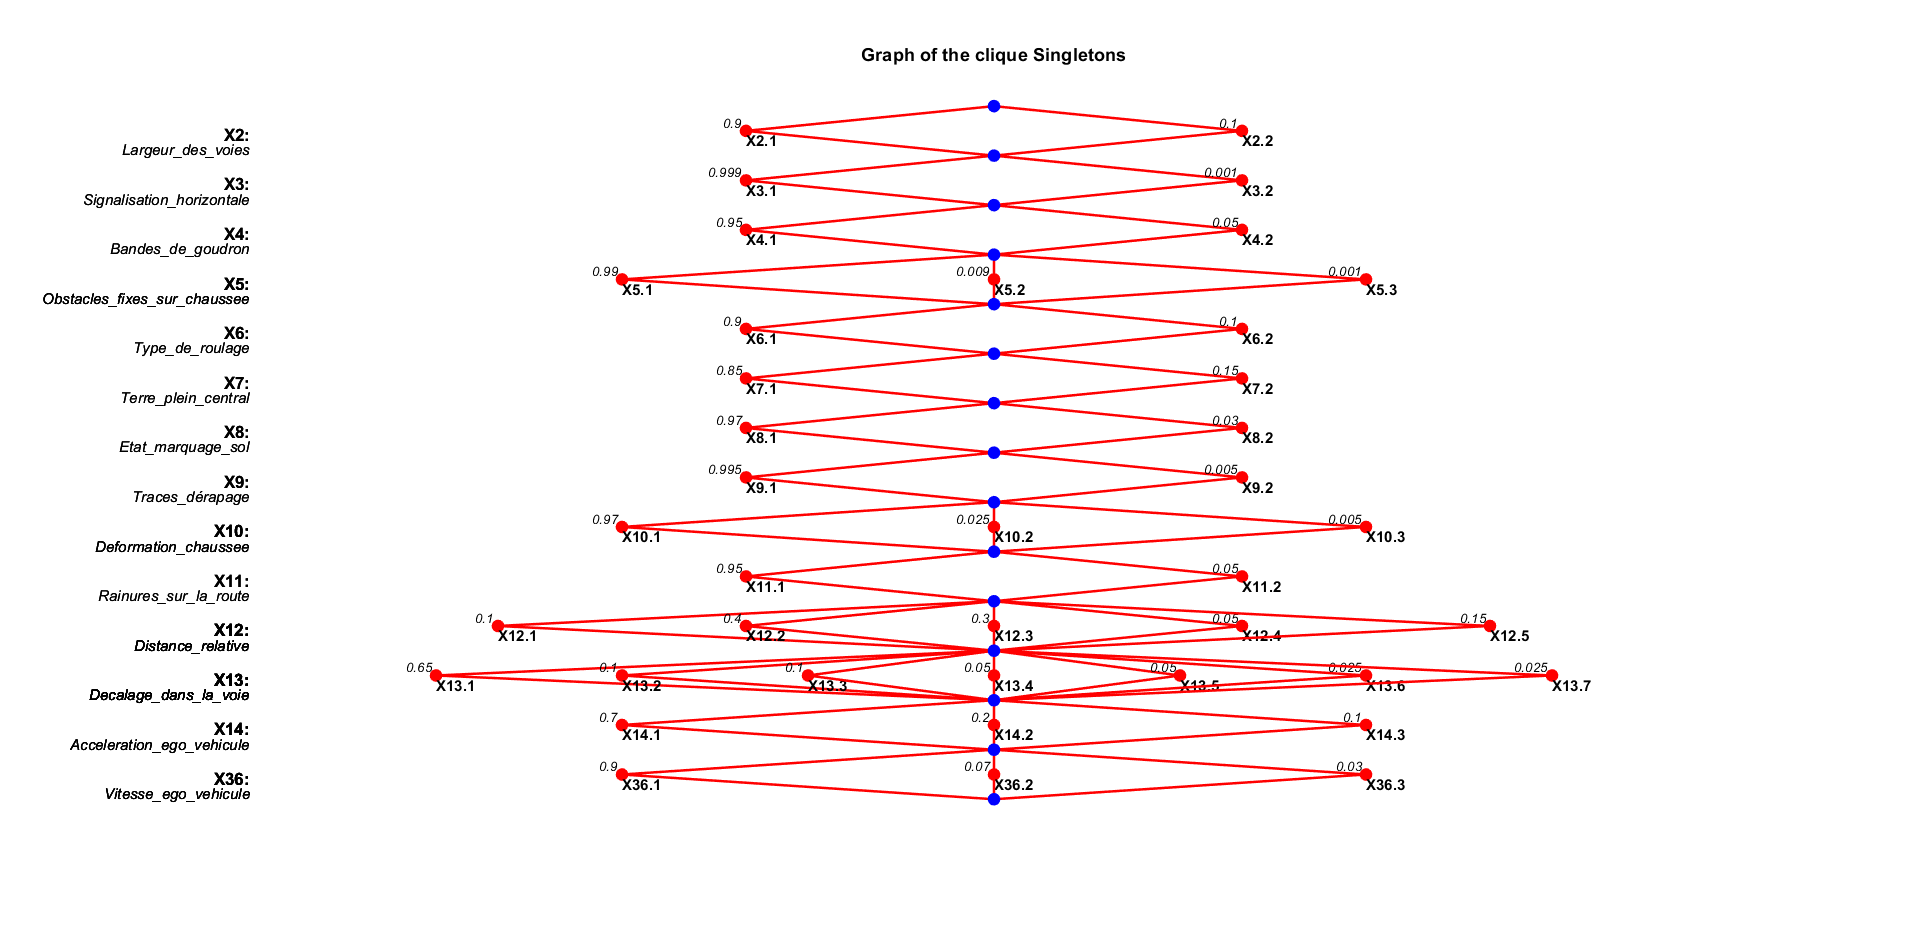
\includegraphics[width=0.8\linewidth]{../../assets/images/fig_Singletons.png}
    \caption{Sơ đồ quyết định cho dữ liệu Singleton}
\end{figure}

\begin{figure}[h!]
    \centering
    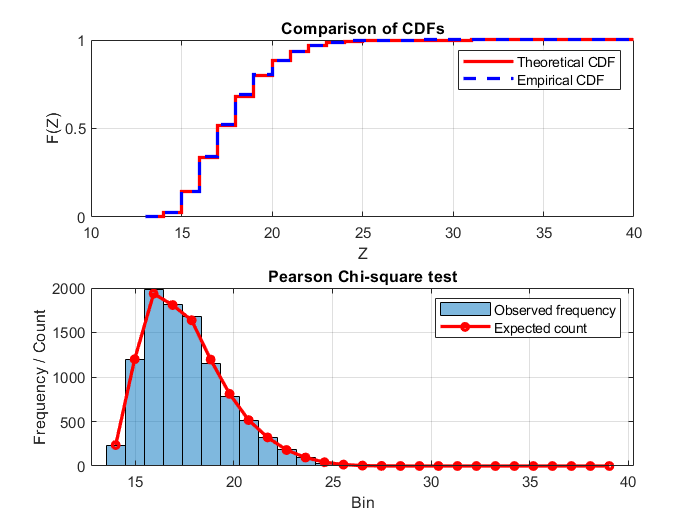
\includegraphics[width=0.8\linewidth]{../../assets/images/KS_fig_Singletons.png}
    \caption{Kết quả kiểm định Kolmogorov-Smirnov cho dữ liệu Singletons}
\end{figure}

\subsection{Kiểm định Pearson và Kolmogorov-Smirnov kết hợp}

\begin{matlab}
\begin{lstlisting}
function [Dn, dn, h_ks, p_ks, ksstat, cv_ks, chi2stat, p_chi2, chi2_crit] = ...
    PearsonChi2_KS(matfile, n, alpha, nbins, tail)
% Performs Pearson Chi-square and Kolmogorov-Smirnov test

% Load theoretical distribution
load(matfile, 'Z_vals', 'PZ', 'FZ');

% Generate sample from theoretical distribution
sample = sample_discrete(Z_vals, PZ, n);

% Perform Pearson Chi-square test
[chi2stat, df, p_chi2, O, E] = pearson_gof_test(Z_vals, PZ, n, nbins);
chi2_crit = chi2inv(1-alpha, df);

% Perform Kolmogorov-Smirnov test
[h_ks, p_ks, ksstat, cv_ks] = kstest(sample, ...
    @(x) interp1(Z_vals, FZ, x, 'linear', 0), ...
    'Alpha', alpha, 'Tail', tail);

% Compute detailed KS statistics
[f_emp, x_emp] = ecdf(sample);
f_theo = interp1(Z_vals, FZ, x_emp, 'linear', 0);

% Supremum statistic
Dn = max(abs(f_emp - f_theo));

% Integrated statistic (Cramér-von Mises type)
dn = trapz(x_emp, (f_emp - f_theo).^2);

% Display results
fprintf('=== KIỂM ĐỊNH PEARSON CHI-SQUARE ===\n');
fprintf('Chi-square statistic: %.4f\n', chi2stat);
fprintf('Degrees of freedom: %d\n', df);
fprintf('P-value: %.6f\n', p_chi2);
fprintf('Critical value (α=%.3f): %.4f\n', alpha, chi2_crit);

fprintf('\n=== KIỂM ĐỊNH KOLMOGOROV-SMIRNOV ===\n');
fprintf('KS statistic: %.6f\n', ksstat);
fprintf('P-value: %.6f\n', p_ks);
fprintf('Critical value: %.6f\n', cv_ks);
fprintf('Supremum distance: %.6f\n', Dn);
fprintf('Integrated distance: %.6f\n', dn);
end
\end{lstlisting}
\end{matlab}

\begin{figure}[h!]
    \centering
    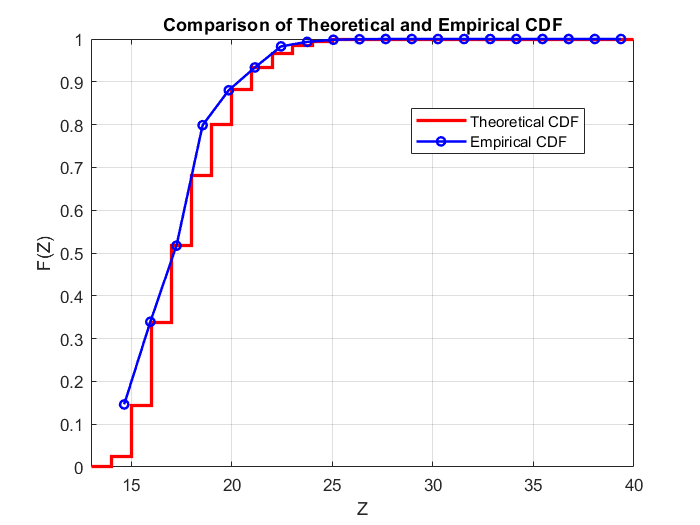
\includegraphics[width=0.8\linewidth]{../../assets/images/Singletons_Pearson.png}
    \caption{Kết quả kiểm định Pearson cho dữ liệu Singletons}
\end{figure}

\section{Ứng dụng với các tập dữ liệu khác}

\subsection{Phân tích dữ liệu Binaires}

\begin{figure}[h!]
    \centering
    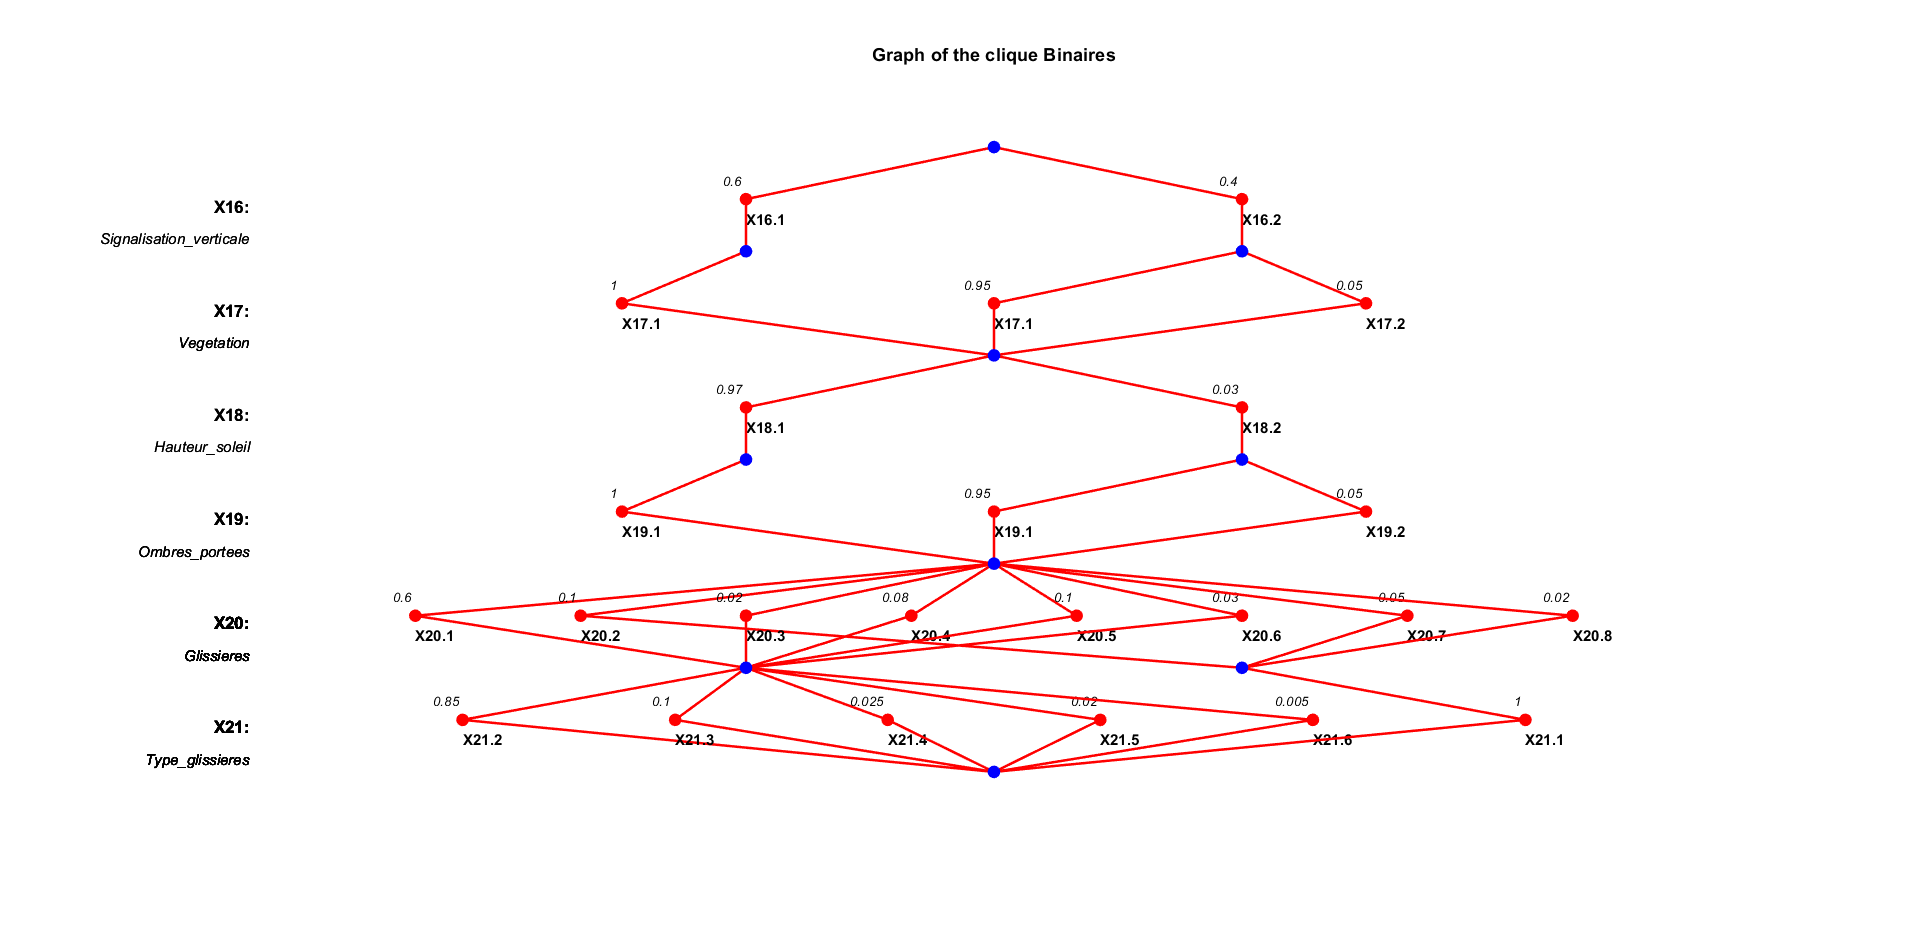
\includegraphics[width=0.8\linewidth]{../../assets/images/fig_Binaires.png}
    \caption{Sơ đồ phụ thuộc cho dữ liệu Binaires}
\end{figure}

\subsection{Phân tích dữ liệu Meteo}

\begin{figure}[h!]
    \centering
    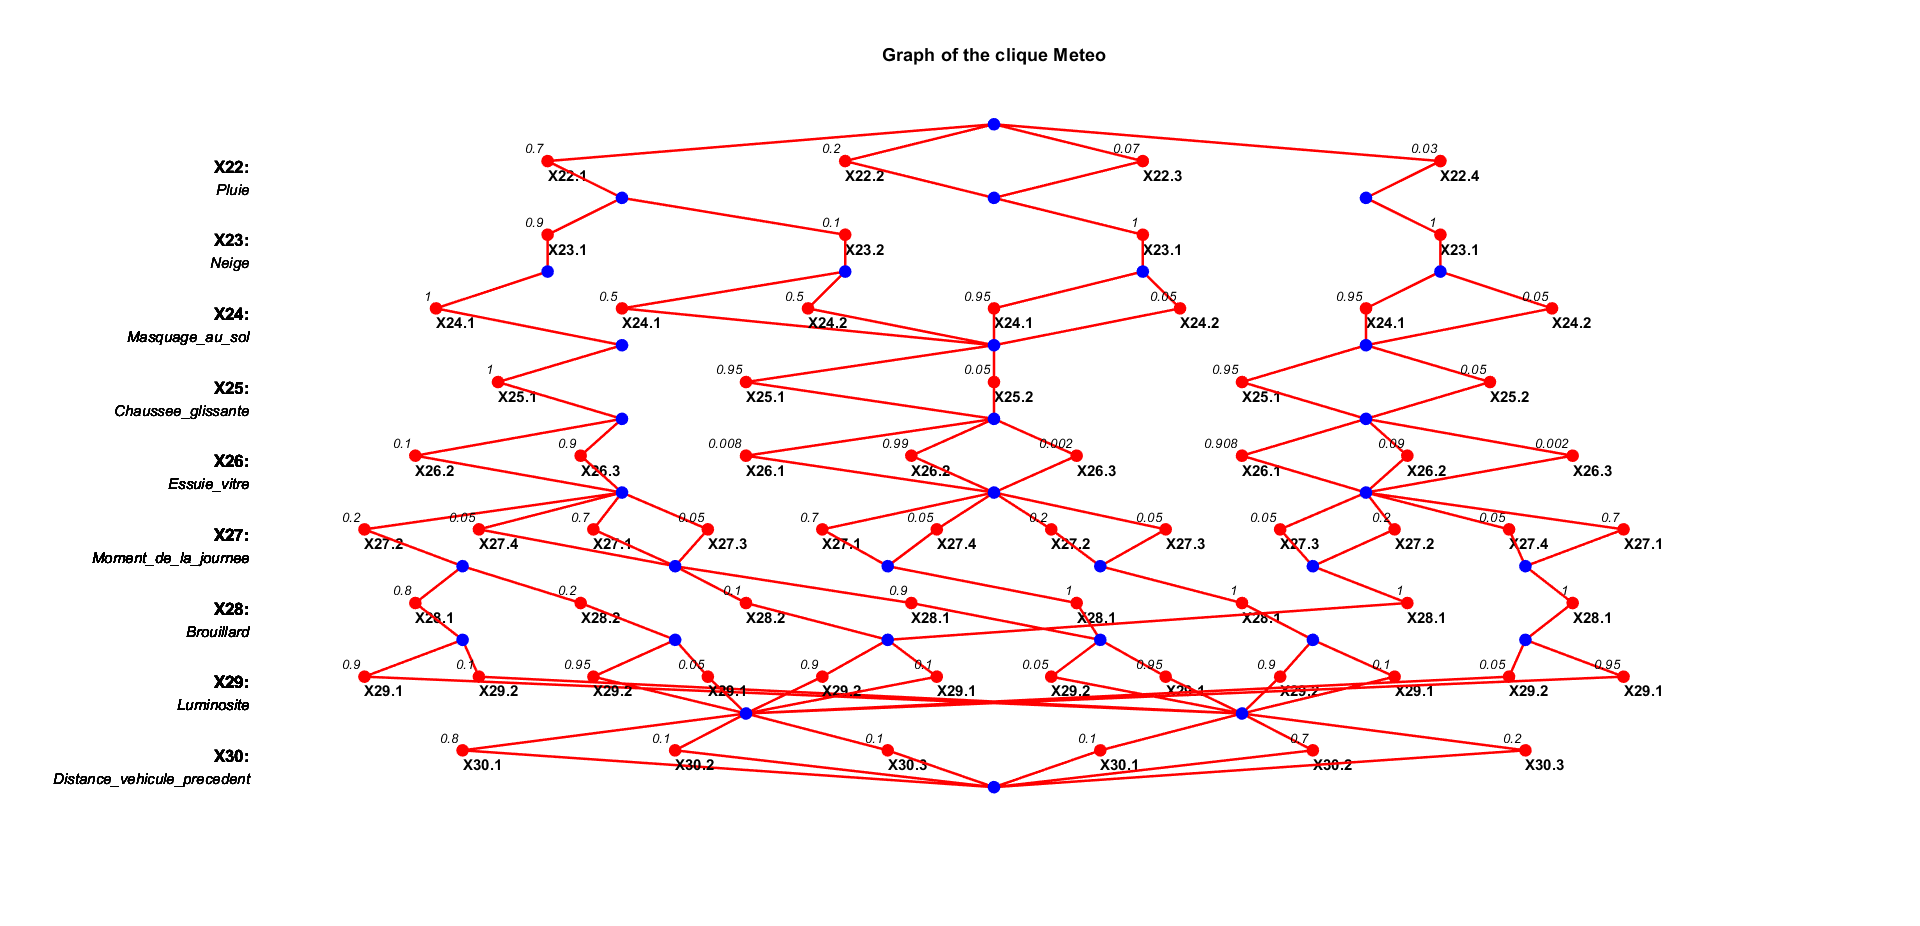
\includegraphics[width=0.8\linewidth]{../../assets/images/fig_Meteo.png}
    \caption{Sơ đồ phụ thuộc cho dữ liệu khí tượng}
\end{figure}

\subsection{So sánh kết quả kiểm định}

\begin{figure}[h!]
    \centering
    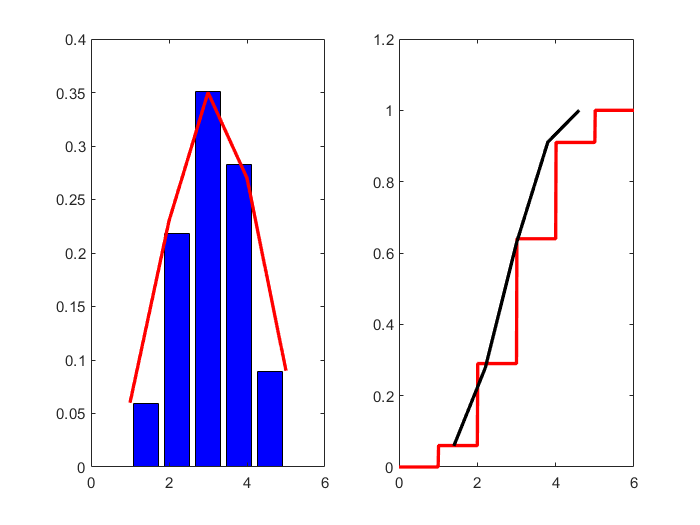
\includegraphics[width=0.8\linewidth]{../../assets/images/X_Y_PTest.png}
    \caption{So sánh kết quả kiểm định Pearson giữa các biến X và Y}
\end{figure}

\subsection{Ứng dụng trong phân tích dữ liệu thực tế}
\subsubsection*{Dữ liệu chất lượng sản phẩm}
Xét bài toán kiểm soát chất lượng trong sản xuất, với các biến:
\begin{itemize}
    \item Kích thước sản phẩm (liên tục)
    \item Loại máy sản xuất (định danh)
    \item Ca làm việc (thứ tự)
    \item Chất lượng (nhị phân: đạt/không đạt)
\end{itemize}

\begin{figure}[h!]
    \centering
    
\includegraphics[width=.8\linewidth]{../../assets/logos/university-logo.png}
    \caption{Sơ đồ mô hình kiểm soát chất lượng}
\end{figure}

\subsubsection*{Quy trình phân tích}
\begin{enumerate}
    \item Kiểm định tính chuẩn của kích thước sản phẩm (Shapiro-Wilk)
    \item Kiểm định sự độc lập giữa máy và ca làm việc (Chi-square)
    \item So sánh chất lượng giữa các máy (Kruskal-Wallis)
    \item Phân tích tương quan giữa kích thước và chất lượng (Spearman)
\end{enumerate}

\subsection{Kiểm định trên mô hình tổng hợp}
Sau khi có các kết quả kiểm định riêng lẻ, cần kết hợp để đưa ra kết luận tổng thể về hệ thống sản xuất.

\subsubsection*{Điều chỉnh đa so sánh}
Khi thực hiện nhiều kiểm định đồng thời, cần điều chỉnh mức ý nghĩa để kiểm soát tỷ lệ sai lầm:

\begin{itemize}
    \item \textbf{Bonferroni}: $\alpha' = \frac{\alpha}{m}$ với $m$ là số kiểm định
    \item \textbf{Holm}: Sắp xếp p-values tăng dần và so sánh với $\frac{\alpha}{m+1-i}$
    \item \textbf{Benjamini-Hochberg}: Kiểm soát False Discovery Rate (FDR)
\end{itemize}

\begin{figure}[h!]
    \centering
    
\includegraphics[width=.8\linewidth]{../../assets/logos/university-logo.png}
    \caption{Biểu đồ so sánh các phương pháp điều chỉnh đa so sánh}
\end{figure}

\section{Kết luận chương}

Chương này đã trình bày chi tiết các phương pháp kiểm định thống kê quan trọng, từ những kiểm định cơ bản như Pearson chi-square và Kolmogorov-Smirnov đến các kiểm định tiên tiến hơn như Anderson-Darling và các kiểm định phi tham số. 

Những điểm chính cần ghi nhớ:
\begin{itemize}
    \item Mỗi kiểm định có điều kiện áp dụng và giả định riêng
    \item Kiểm định phi tham số mạnh mẽ hơn nhưng ít hiệu quả hơn khi giả định được thỏa mãn
    \item Cần cẩn thận với vấn đề đa so sánh và điều chỉnh mức ý nghĩa phù hợp
    \item Mô phỏng Monte Carlo là công cụ hữu ích để đánh giá và so sánh hiệu quả của các kiểm định
\end{itemize}

Các phương pháp này tạo nền tảng vững chắc cho việc phân tích dữ liệu trong thực tiễn và chuẩn bị cho các kỹ thuật phân tích nhiều chiều sẽ được trình bày trong chương tiếp theo.
